\chapter{Discussion}
Please tell more about conclusion and how to the next work of this study.

\maxdeadcycles=200
\extrafloats{100}

\section{Cokro Edi Prawiro / 1164069}
\subsection{Teori}

\begin{enumerate}

\item Jelaskan kenapa file suara harus dilakukan MFCC dilengkapi dengan ilustrasi atau gambar.\par
digunakan untuk mengidentifikasi jenis suara misalkan jenis suara gendre lagu jes pop metal dan klasikal atau suara ultra sonic untuk contohnya dapat di gambar \ref{c113} 

\begin{figure}[!htbp]
      \centering{
\includegraphics[width=0.7\textwidth]
      {figures/cokro/c113}}
      \caption{Ilustrasi gambar metode MFCC}
      \label{c113}
      \end{figure}

\item Jelaskan konsep dasar neural network. dilengkapo dengan ilustrasi gambar. \par
konsep neural network dilaka ada inputan pasti ada outputan sesuai dengan kategori inputan dan fungsi di dalamnya. untuklebih jelasnya dapat dilihat pada ilustrasi gambar berikut. \ref{c114}

\begin{figure}[!htbp]
      \centering{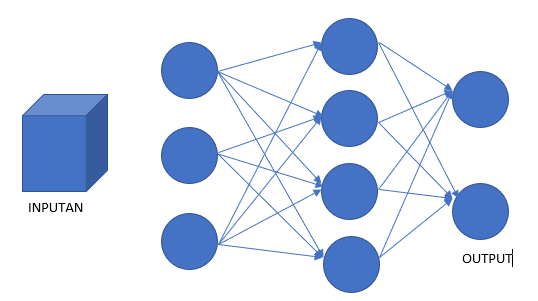
\includegraphics[width=0.7\textwidth]
      {figures/cokro/c114}}
      \caption{Ilustrasi Konsep dasar neural network}
      \label{c114}
      \end{figure}

\item Jelaskan konsep pembobotan  dalam neural network. dilengkapidengan ilustrasi gambar. \par
pembobotan dalam neural network yaitu digunakan untuk membedakan objek inputan atau variabel inputan untuk AI misalkan apel dan jeruk digunakan untuk variabel inputan maka dibuat pembobotan anatara kedua benda tersebut untuk menentukan output yang pasti dari inputan yang dilakukan untuk lebih jelasnya dapat dilihat pada gambar. \ref{c115}

\begin{figure}[!htbp]
      \centering{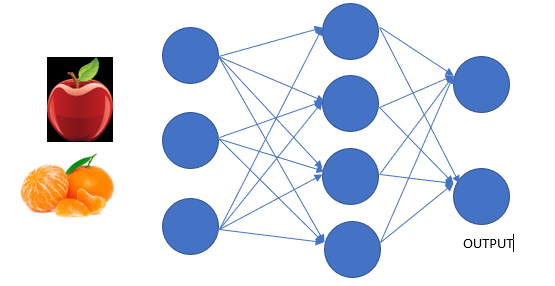
\includegraphics[width=0.7\textwidth]
      {figures/cokro/c115}}
      \caption{Ilustrasi Konsep pembobotan pada neural network}
      \label{c115}
      \end{figure}

\item Jelaskan konsep aktifitas dalam neural network. dilengkapi dengan ilustrasi gambar.\par

cara aktifitas dalam neural network dilakukan terhadap input pada neural network inputan tersebut dimasukan kepada fungsi pada mesin misalkan fungsi tanh(x) sehingga di hasilkanlah output yang sesuai dengan fungsi tersebut. untuk lebih jelasnya dapat dilihat pada gambar \ref{c116}

\begin{figure}[!htbp]
      \centering{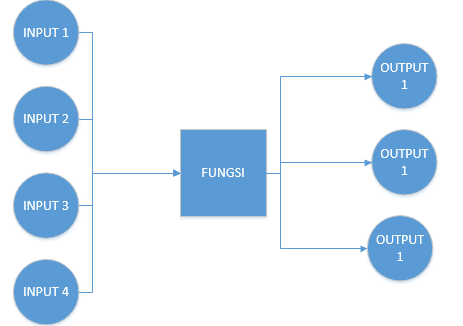
\includegraphics[width=0.7\textwidth]
      {figures/cokro/c116}}
      \caption{Gambar yang dibaca hasil plotnya}
      \label{c116}
	   \end{figure}

\item Jelaskan cara membaca hasil plot dari MFCC dilengkapi dengan ilustrasi gambar. \par
cara membaca hasil ploting dari MFCC yaitu tentukan terlebih dahulu batas minimal Hz dari gelombang suara dan batas maksimal dari suara tersebut. kemudian warna yang paling pekat merupakan hasil dari pengolahan data tersebut misalkan muncul warna orange pekat di bagian bawah dan orange muda di bagian atas yang berarti suara tersebut kuat bagian basnya dan biasanya juga antara warna yang pekat tersebut ada jarak. untuk lebih jelasnya dapat di lihat pada gambar \ref{c117} berikut.

\begin{figure}[!htbp]
      \centering{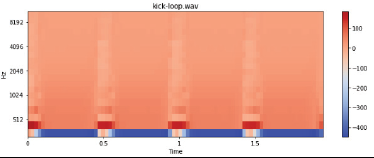
\includegraphics[width=0.7\textwidth]
      {figures/cokro/c117}}
      \caption{Ilustrasi Cara Membaca Hasil Plot}
      \label{c117}
      \end{figure}

\item Jelaskan apa itu one-hot encoding, dilengkapi dengan ilustrasi kode atau gambar.\par
one-hot encoding merupakan pemberian nilai pada suatu variabel jika nilai itu iya maka nilainya satu dan jika tidak maka nilainya nol untuk lebih jelasnya dapat dilihat pada gambar \ref{c118} tersebut

\begin{figure}[!htbp]
      \centering{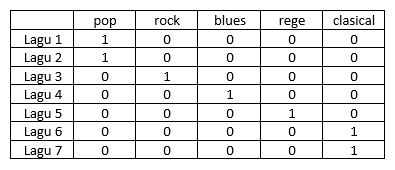
\includegraphics[width=0.7\textwidth]
      {figures/cokro/c118}}
      \caption{Ilustrasi Konsep one-hot encoding}
      \label{c118}
      \end{figure}

\item Jelaskan apa dari np.unique dan to\_categorical dalam kode program, dilengkapi dengan ilustrasi atau gambar.\par
digunakan untuk membuat array sedangkan  to\_categorical digunakan untuk membuat matrix baui itu 64 bit atau 32 bit. untuk contoh gambarnya dapat dilihat pada gambar \ref{c119} dan gambar \ref{c120}

\begin{figure}[!htbp]
      \centering{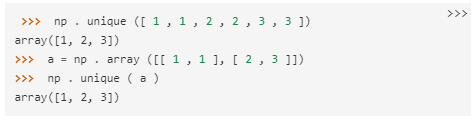
\includegraphics[width=0.7\textwidth]
      {figures/cokro/c119}}
      \caption{Ilustrasi  np.unique}
      \label{c119}
      \end{figure}

\begin{figure}[!htbp]
      \centering{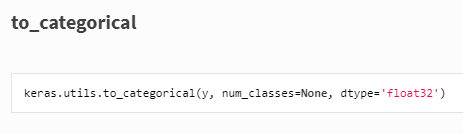
\includegraphics[width=0.7\textwidth]
      {figures/cokro/c120}}
      \caption{Ilustrasi to\_categorical}
      \label{c120}
      \end{figure}

\item Jelaskan apa fungsi dari Sequential dalam kode program, dilengkapi dengan ilustrasi atau gambar. \par
sequential adalah prosesperbandingan setiap elemen satu persatu mulai dari dari objek pertama hingga yang di tuju atau jika mencari angka 100 maka sequential akan membagi bagian misalnya dari satu sampai 20 dan seterusnya sampai mendapat nilai seratus. untuk lebih jelasnya dapat dilihat gambar \ref{c}  berikut:

\begin{figure}[!htbp]
      \centering{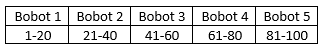
\includegraphics[width=0.5\textwidth]
      {figures/cokro/c121}}
      \caption{Ilustrasi Konsep pembobotan pada neural network}
      \label{c121}
      \end{figure}
\end{enumerate}

\subsection{Praktikum}
\begin{enumerate}
\item Jelaskan isi dari data GTZAN Genre Collection dan data dari freesound. Buat kode program program untuk meload data tersebut untuk digunakan pada MFCC. Jelaskan arti dari perbaris kode yang dibuat (harus beda dengan teman satukelas).\par
\subitem Isi data data merupakan datasets lagu atau suara yang tersiri dari 10 gendre yang di simpan kedalam 10 folder yaitu folder blues, classical, country, disco, hiphop, jazz, metal, pop, reggae, dan rock ke sepuluh folder tersebut masing-masing  berisi 100 data suara sedangkan data freesound merupakan contoh data suara yang akan di gunakan untuk menguji hasil pengolahan data tersebut dengan menggunakan metode mfcc. apakah suara dari freesound termasuk kategori jazz pop atau sebagainya ?.

\lstinputlisting[firstline=1, lastline=21]{src/cokro/praktikum6.py}

\subitem dapat dilihat pada kode diatas pada baris kesatu dilakukan import librosa tang digunakan untuk fungsi mfcc pada suara.
pada baris kedua dilakukan import librosa featuse dan pada baris ke tiga dilakukan librosa display selanjutnya pada baris ke empat dilakukan import glob kemudian insert numpy untuk pengolahan data menjadi vektor setelah itu dilakukan import matplotlib untuk melakukan ploting setelah itu dilakukan import librari keras.\par

\subitem Selanjutnya yaitu membuat fungsi mfcc dengan nama display\_mfcc yang didalamnya terdapat variabel y yang berisi method librosa load kemudian variabel mfcc yang berisi method librosa featurea mfcc. Setelah itu membuat flot figure dengan ukuran 10 banding 4 kemudian di isi oleh data librosa display dengan variabel x nya yaitu waktu dan y yaitu mel atau Hz kemudian melakukan plot warna setelah itu melakukan plot judul dan terakhir flot di tampilkan. 

\item Jelaskan perbaris kode program dengan kata-kata dan di lengkapi ilustrasi gambar fungsi dari display\_mfcc().\par

\lstinputlisting[firstline=22, lastline=43]{src/cokro/praktikum6.py}

\subitem pada baris ke dua program diatas digunakan untuk mendisplay tampilan glombang suara dari file 266093\_\_stereo-surgeon\_\_kick-loop-5.wav menggunakan metode mfcc dengan menggunakan fungsi display\_mfcc yang telah tadi di buat pada nomer dua begitu juga pada baris ke 4 6 8 sampai ke 22 secara teksis sama menggunakan fungsi display\_mfcc hanyasaja beda peyimpanan data yang akan di tampilkan atau di eksekusi. untuk contoh hasilnya dapat dilihat pada gambar \ref{c122} berikut:

\begin{figure}[!htbp]
      \centering{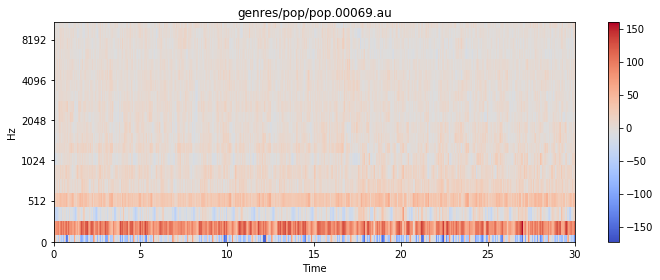
\includegraphics[width=0.5\textwidth]
      {figures/cokro/c122}}
      \caption{Ilustrasi gambar fungsi dari display\_mfcc() }
      \label{c122}
      \end{figure}

Gambar \ref{c122} tersebut merupakan hasil dari mfcc dari salah satu gender lagu pop yang ada pada datasets yang 1000 atau terdapat dalam sepuluh folder tadi.

\item Jelaskan perbaris dengan kata-kata dan dilengkapi dengan ilustrasi gambar fungsi dari extract\_features\_song jelaskan kenapa data yangdiambil merupakan data 25.000 baris pertama ? 

\lstinputlisting[firstline=44, lastline=55]{src/cokro/praktikum6.py}

\subitem pada baris ke tiga di definisikan nama extract\_features\_song yang nantinya akan di gunakan pada fungsi yang lainya kemudian dibuat variabel y dengan method librosa load setelah itu dibuat variabel baru mfcc dengan isi librosa features mfcc dengan isi variabel y tadi kemudian dibuat variabel mfcc dengan isian np.max dan variabel mfcc tadi terakhir di buat array dari data tersebut merupakan data 25000 data pertama. kenapa data 25000 pertama yang digunakan dikarenakan data tersebut digunakan sebagai data testing semakin besar data testing yang di gunakan maka semakin akurat hasil AI. tapi sebenarnya data tersebut relatif bisa lebih besar atau lebih kecil tergantung pada komputer masing masing.

\item Jelaskan Perbaris kode program dengan kata-kata dan di lengkapi ilustrasi gambar fungsi dari generate features and labels.

\lstinputlisting[firstline=56, lastline=76]{src/cokro/praktikum6.py}

\subitem pada baris ke tiga merupakan pendefinisian nama fungsi yaitu generate features and labels kemudian membuat variabel baru dengan array kosing yaitu all\_features dan all\_labels kemudian mendefinisikan isian label untuk gendre dengan cara membuat variabel genres kemudian di isi dengan 10 gendre yang tadi setelah itu dilakukan fungsi if else dengan code for dan in setelah itu akan di buat encoding untuk data tiap tiap label contoh untuk blues 1000000000 dan untuk clasical 0100000000.

\item Jelaskan dengan kata dan praktek kenapa penggunaan fungsi generate features and labels sangat lama saat meload dataset gendre tunjukan keluarannya dari komputer sendiri dan artikan maksud dari luaran tersebut.\par

halnini menjadi lama dikarenakan mesin membaca satupersatu file yang ada pada folder dan dalam foldertersebut terdapat 100 file sehingga wajar menjadi lama ditambah lagi mengolah data yang tadinya suara menjadi bentuk vektor. berikut merupakan codenya.
\lstinputlisting[firstline=77, lastline=79]{src/cokro/praktikum6.py}
kemudian untuk hasilnya dapat dilihat pada gambar \ref{c123} berikut :

\begin{figure}[!htbp]
      \centering{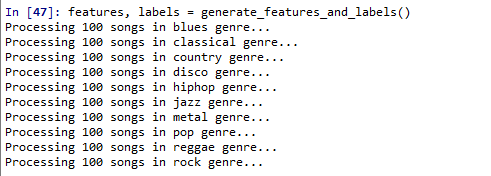
\includegraphics[width=0.5\textwidth]
      {figures/cokro/c123}}
      \caption{Hasil dari fungsi generate features and labels}
      \label{c123}
      \end{figure}

pada keluaran yang terdapat pada gambar \ref{c123} tersebut menunjukan bahwa mesin telah meload dan membaca masing masing 100 data dari setiap gendre

\item jelaskan kenapa harus dilakukan pemisahan data training dan data testing sebesar 80 persen praktekan dengan kode dan tunjukan keluarannya dari komputer sendiri dan artikan maksud dari luaran tersebut. 

untuk code nya adalah sebagai berikut  yang merupakan code untuk membagi data sebanyak 80 persen untuk data training maka data musik tadi yang total jumlahnya 1000 akan di bagi dua untuk data training sebanyak 800  dan 200 untuk data testing.

\lstinputlisting[firstline=83, lastline=84]{src/cokro/praktikum6.py}

dan untuk hasilnya dapat dilihat pada gambar \ref{c124} dan gambar \ref{c125} pada gambar tersebut menunjukan hasil dari pembagian 80 persen tadi dimana kolom menjadi 25010 yangmerupakan kombinasi antara label dan data 25000 yang diambil dari data pertama.

\begin{figure}[!htbp]
      \centering{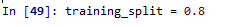
\includegraphics[width=0.5\textwidth]
      {figures/cokro/c124}}
      \caption{Hasi eksekusi code}
      \label{c124}
      \end{figure}

\begin{figure}[!htbp]
      \centering{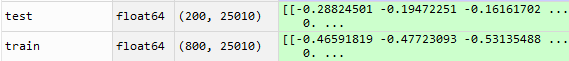
\includegraphics[width=0.5\textwidth]
      {figures/cokro/c125}}
      \caption{Hasil pembagian 80 persen}
      \label{c125}
      \end{figure}

\item praktekan dan jelaskan masing masing parameter dari fungsi Sequential().  tunjukan keluarannya dari komputer sendiri dan artikan maksud dari luaran tersebut.\par
\subitem fungsi sequential digunakan untuk mengolah data inputan sesuai dengan fungsi yang ada pada fungsi sequential pada fungsi sequential kali ini menggunakan dua fungsi dapat dilihat pada gambar \ref{c126} pada gambar tersebut fungsi sequential mengkompile data dari 100 neuron atau dari 1 folder file dengan menggunakan fungsi relu dan softmax untuk menghasilkan outputan yang sesuai dengan keriteria.
\lstinputlisting[firstline=105, lastline=111]{src/cokro/praktikum6.py}

\begin{figure}[!htbp]
      \centering{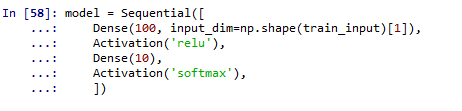
\includegraphics[width=0.5\textwidth]
      {figures/cokro/c126}}
      \caption{Hasil fungsi sequential}
      \label{c126}
      \end{figure}

\item praktekan dan jelaskan masing masing parameter dari fungsi compile().  tunjukan keluarannya dari komputer sendiri dan artikan maksud dari luaran tersebut. \par
\subitem yaitu fungsi kompile yang digunakan untuk mengetahui parameter yang digunakan dari data yang telah diolah untuk caranya dapat menggunakan codingan sebagai berikut dan untuk hasilnya dapat dilihat pada gambar \ref{c127} pada gambar tersebut memunculkan parameternya berapasaja dan total parameter yang digunakan.

\lstinputlisting[firstline=112, lastline=116]{src/cokro/praktikum6.py}

\begin{figure}[!htbp]
      \centering{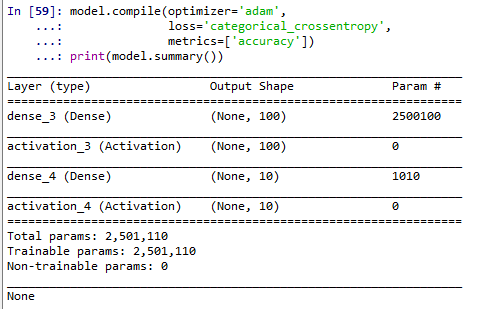
\includegraphics[width=0.5\textwidth]
      {figures/cokro/c127}}
      \caption{Hasil fungsi compile}
      \label{c127}
      \end{figure}

\item praktekan dan jelaskan masing masing parameter dari fungsi fit().  tunjukan keluarannya dari komputer sendiri dan artikan maksud dari luaran tersebut.\par
\subitem pada fungsi ini dilakukan pengolahan data dari 10 label tadi atau 10 file data sets tadi kemudian di hitung tingkat akurasi masing masing dan tingkat kegagalan atau loss data darisetiap file tersebut caranya dengan melakukan codingan berikut. dan untuk hasilnya dapat dilihat pada gambar \ref{c128} berikut pada gambar tersebut menunjukan 10 pengolahan data untuk menentukan nilai akurasi dan loss dari data tersebut dan selanjutnya dilakukan fingsi evaluasi.

\lstinputlisting[firstline=117, lastline=119]{src/cokro/praktikum6.py}

\begin{figure}[!htbp]
      \centering{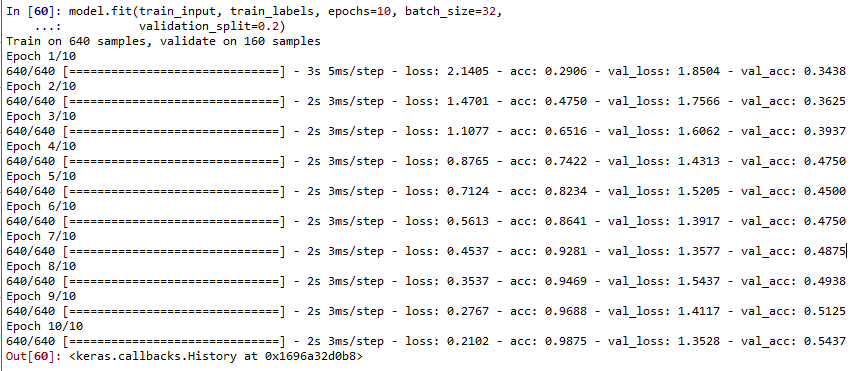
\includegraphics[width=0.5\textwidth]
      {figures/cokro/c128}}
      \caption{Hasil fungsi fit}
      \label{c128}
      \end{figure}

\item praktekan dan jelaskan masing masing parameter dari fungsi evaluate().  tunjukan keluarannya dari komputer sendiri dan artikan maksud dari luaran tersebut.\par
\subitem pada fungsi ini dilakukan evaluasi terhadap datayang telah di runing sebelummnya untuk lebih jelasnya dapat di lihat codingan tersebut  pada codingan tersebut dilakukan evaluasi pada tingkat kegagalan dan akurasi kebenaran maka hasilnya dapat dilihat pada gambar \ref{c129} pada gambar tersebut di munculkan hasil evaluasi dari 10 proses dari setiap gendre yaitu akurasi sebesar 51 persen dan loss data sebesar 1.4105 data.

\lstinputlisting[firstline=120, lastline=125]{src/cokro/praktikum6.py}

\begin{figure}[!htbp]
      \centering{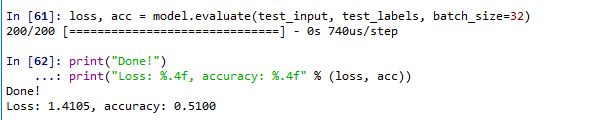
\includegraphics[width=0.5\textwidth]
      {figures/cokro/c129}}
      \caption{Hasil fungsi evaluasi}
      \label{c129}
      \end{figure}

\item praktekan dan jelaskan masing masing parameter dari fungsi predic  tunjukan keluarannya dari komputer sendiri dan artikan maksud dari luaran tersebut. \par 
\subitem fungsi predic merupakan fungsi untuk membandingkan tingkat akurasi pada setiap label yang sepuluh tadi maka data akan di sandingkan ke masing masing tingkat akurasinya, yang akurasinya paling tinggi maka itulah jawaban untuk setiap inputan yang dilakukan. 

\lstinputlisting[firstline=126, lastline=127]{src/cokro/praktikum6.py}

\begin{figure}[!htbp]
      \centering{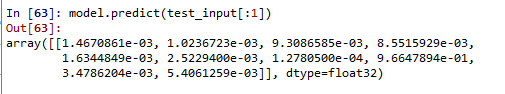
\includegraphics[width=0.5\textwidth]
      {figures/cokro/c130}}
      \caption{Hasil fungsi prediksi}
      \label{c130}
      \end{figure}

untuk hasilnya dapat dilihat pada gambar \ref{c130} yang menunukan hasil berupa array dari kesepuluh label yang telah di olah tadi.
\end{enumerate}


\section{Fathi Rabbani / 1164074}
\subsection{Teori}
\begin{enumerate}
\item Kenapa file suara harus dilakukan MFCC
\subitem MFCC digunakan untuk mengidentifikasi jenis suara yang dimasukan seperti suara lagu, hujan atau pun suara yang tidak dapat didengar oleh telinga manusia yaitu Ultrasonik, sehingga dibutuhkan penggunaan MFCC untuk memproses data tersebut agar dapat dibaca oleh manusia. ilustrasi untuk MFCC dapat dilihat pada gambar \ref{data1}

\begin{figure}[!htbp]
      \centering{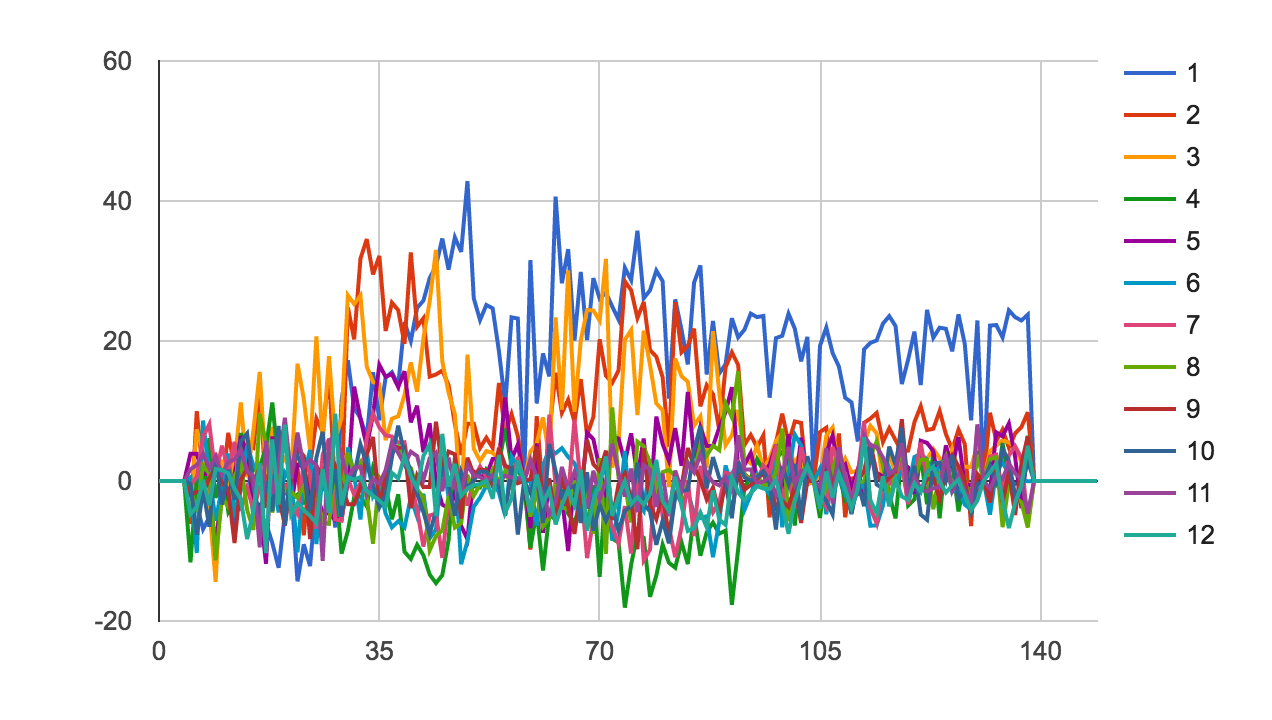
\includegraphics[width=0.5\textwidth]{figures/fathi/chapter6/hari1/1}}
      \caption{Ilustrasi MFCC}
      \label{data1}
\end{figure}

\item Konsep dasar Neural Network
\subitem Neural Network sebenarnya mengadopsi dari kemampuan otak manusia yang mampu memberikan stimulasi/rangsangan, melakukan proses, dan memberikan output. Output diperoleh dari variasi stimulasi dan proses yang terjadi di dalam otak manusia.
ilustrasi Neural Network dapat dilihat pada gambar \ref{data2}

\begin{figure}[!htbp]
      \centering{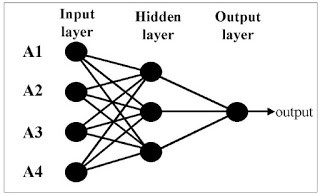
\includegraphics[width=0.5\textwidth]{figures/fathi/chapter6/hari1/2}}
      \caption{Ilustrasi Neural Network}
      \label{data2}
\end{figure}

\item Konsep Pembobotan dalam Neural Network
\subitem konsep pembobotan dalam neural network digunakan untuk membedakan data satu dengan data lainnya, sebagai contoh dapat dilihat pada gambar \ref{data3}. dimana data inputan yang masuk adalah 2 data yaitu "anjing" dan "kucing" yang diolah dengan proses membandingkan data dan diolah melalui pembobotan sehingga menampilkan hasil output.

\begin{figure}[!htbp]
      \centering{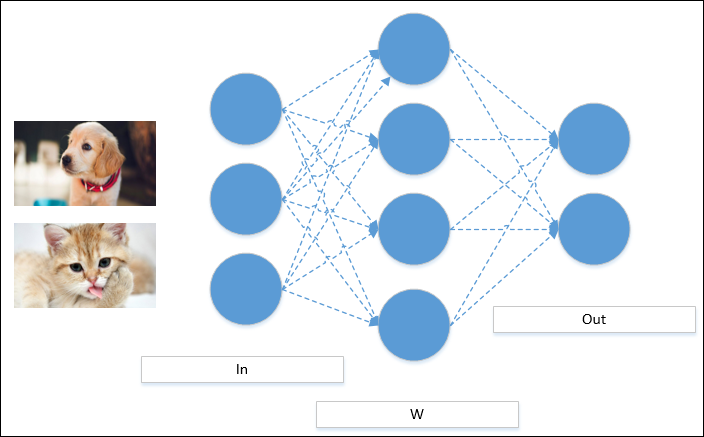
\includegraphics[width=0.5\textwidth]{figures/fathi/chapter6/hari1/3}}
      \caption{Ilustrasi pembobotan Neural Network}
      \label{data3}
\end{figure}

\item Konsep Aktifasi dalam Neural Network
\subitem dalam Neural Network fungsi aktifasi meliputi inputan dan diproses sehingga menghasilkan Output nilai yang diharapkan, dengan menggunakan persepsi alur cara penyampaian informasi pada jaringan syaraf otak. ilustrasi dapat dilihat pada gambar \ref{data4}

\begin{figure}[!htbp]
      \centering{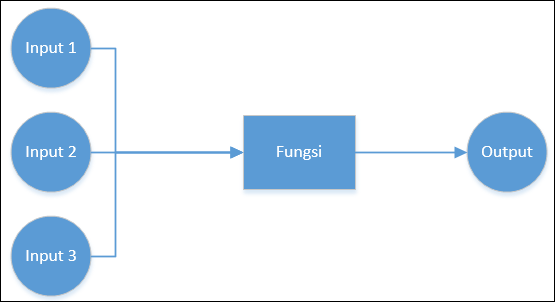
\includegraphics[width=0.5\textwidth]{figures/fathi/chapter6/hari1/4}}
      \caption{Ilustrasi fungsi aktifasi Neural Network}
      \label{data4}
\end{figure}

\item cara membaca hasil PLOT dari MFCC

\begin{figure}[!htbp]
      \centering{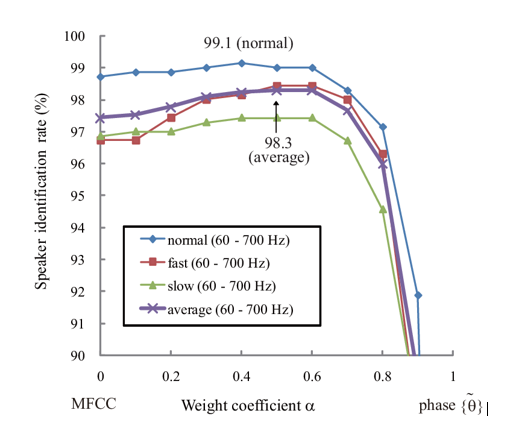
\includegraphics[width=0.5\textwidth]{figures/fathi/chapter6/hari1/5}}
      \caption{Ilustrasi Membaca nilai Plot dari MFCC}
      \label{data5}
\end{figure}

\item One-hot Encoding
\subitem penggunaan One-hot Encoding adalah dengan membaca data yang memiliki nilai 1 sebagai nilai tinggi atau bisa disebut juga sebagai nilai positif dan 0 sebagai nilai rendah yang bermakna juga sebagai nilai negatif. ilustrasi dapat dilihat pada gambar \ref{data6}

\begin{figure}[!htbp]
      \centering{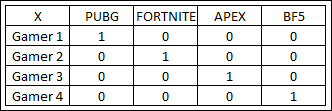
\includegraphics[width=0.5\textwidth]{figures/fathi/chapter6/hari1/6}}
      \caption{Ilustrasi One-hot Encoding}
      \label{data6}
\end{figure}

\item fungsi dari np.unique dan to\_categorial dalam Code Program
\subitem fungsi dari NP.UNIQUE dalah untuk membuat data elemen menjadi nilai yang bersifat unik dalam artian (Array), ilustrasi dapat dilihat pada gambar \ref{data7}

\begin{figure}[!htbp]
      \centering{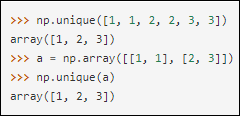
\includegraphics[width=0.5\textwidth]{figures/fathi/chapter6/hari1/7}}
      \caption{Ilustrasi np.unique}
      \label{data7}
\end{figure}

\subitem sedangkan perintah to\_categorial adalah untuk membuat data integer yang terdeteksi untuk diubah menjadi data matrix biner. ilustrasi dapat dilihat pada gambar \ref{data8}

\begin{figure}[!htbp]
      \centering{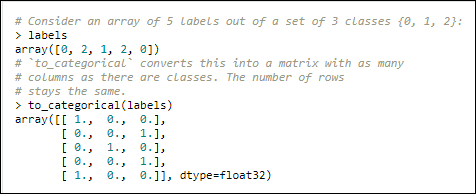
\includegraphics[width=0.5\textwidth]{figures/fathi/chapter6/hari1/8}}
      \caption{Ilustrasi to\_categorial}
      \label{data8}
\end{figure}

\item fungsi dari Sequential
\subitem fungsi dari Sequential dari code program adalah untuk membagi data - data agar dapat dianalisis oleh sistem lebih mudah, misalkan dari data 100 dibagi prosesnya menjadi 4 yaitu 25 perproses, seperti yang terdapat pada gambar \ref{data9} sehingga hasil yang didapatkan akan lebih baik lagi.

\begin{figure}[!htbp]
      \centering{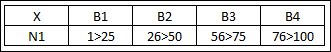
\includegraphics[width=0.5\textwidth]{figures/fathi/chapter6/hari1/9}}
      \caption{Ilustrasi fungsi Sequential}
      \label{data9}
\end{figure}
\end{enumerate}

\subsection{Praktikum}
\begin{enumerate}
\item Penjelasan data GTZAN Genre Collection dan Freesound, Buat Code Program untuk Load data Tersebut.
\subitem GTZAN Genre Collection merupakan datasets yang berisi data lagu yang terdiri dari 10 genre yaitu :
\begin{itemize}
\item Blues
\item Classical
\item Country
\item Disco
\item Hip-Hop
\item Jazz
\item Metal
\item Pop
\item Reggae
\item Rock
\end{itemize}
10 genre tersebut memiliki data sebesar 100 data suara.

\subitem sedangkan Freesound merupakan sebuah contoh suara yang digunakan untuk menguji hasil dari pengolahannya dengan menggunakan metode MFCC, untuk mencari genre yang pas bagi contoh suara tersebut.

\begin{figure}[!htbp]
      \centering{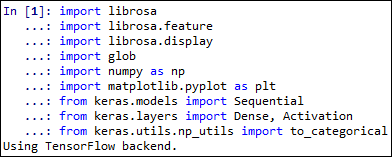
\includegraphics[width=0.5\textwidth]{figures/fathi/chapter6/hari2/1}}
      \caption{Code Program pemanggilan Library}
      \label{data10}
\end{figure}

\subitem Code pada gambar \ref{data10} digunakan untuk memanggil library Librosa yang memuat metode Feature dan Display yang akan digunakan untuk memproses data suara tersebut dengan MFCC. lalu Library Glob yang digunakan untuk mencocokan pattern yang spesifik dari data tersebut, Library Numpe yang digunakan untuk membuat data Vector, Library matplotlib yang digunakan untuk membuat data grafik dan Library Keras adalah open-source yang bekerja untuk memproses TensorFlow, CNTK dan Theano, yang didesain untuk melakukan penelitian dengan menggunakan Deep Neural Network.

\item Penjelasan Code Program display\_mfcc

\begin{figure}[!htbp]
      \centering{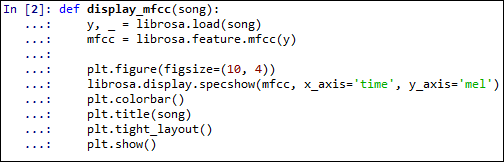
\includegraphics[width=0.5\textwidth]{figures/fathi/chapter6/hari2/2}}
      \caption{Code Program display\_mfcc}
      \label{data11}
\end{figure}

\subitem Code pada gambar \ref{data11} meliputi penggunaan MFCC dengan proses Display yang memiliki penjelasan seabgai berikut, Variable Y berisi Library Librosa dengan method LOAD dan berisi nilai SONG sebagai penggunaan classnya. dan Variable MFCC yang berisi method feature.mfcc dan memiliki nilai dari Variable Y. penggunaan plt sebagai pemanggilan matplotlib dengan method FIGURE yang akan menampilkan data gambar. dan Librosa yang akan menampilkan method display.specshow dengan data dari Variable mfcc dan pengaturan Axis X dan Y. lalu mengisikan data dengan nilai dari COLORBAR, TITLE yang berisi data dari class SONG dan tight\_layout serta show yang akan menampilkan hasil RUN yang dilakukan.

\subitem hasilnya adalah sebagai berikut, dengan menampilkan data dari file disco.00035.au dapat dilihat pada gambar \ref{data12}:

\begin{figure}[!htbp]
      \centering{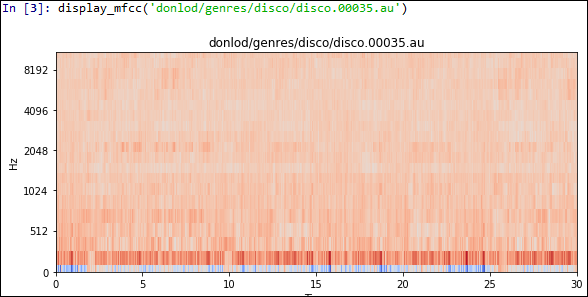
\includegraphics[width=0.5\textwidth]{figures/fathi/chapter6/hari2/3}}
      \caption{Hasil dari Code Program display\_mfcc}
      \label{data12}
\end{figure}

\item Penjelasan Code Program extract\_feature\_song
\subitem Pada Code Program berikut ini akan menjelaskan tentang ekstrasi data feature dari lagu yang akan di olah dengan Code yang ada pada gambar \ref{data13}. dengan menggunakan Variable Y yang berisi method LOAD dengan record datanya dari class F pada extract\_feature\_song lalu membuat Variable mfcc dengan nilai yang akan meload data mfcc dari class Y, lalu melakukan normalisasi pada data Variable mfcc dengan penggunaan np.amax dengan nilai np.absolute(mfcc) lalu melakukan return dengan method np.ndarray.flatten(mfcc)[:25000] dimana data yang akan dibaca adalah sebanyak 25000 data dengan nilainya adalah array.

\begin{figure}[!htbp]
      \centering{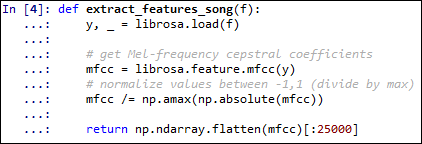
\includegraphics[width=0.5\textwidth]{figures/fathi/chapter6/hari2/4}}
      \caption{Code Program extract\_feature\_song}
      \label{data13}
\end{figure}


\end{enumerate}